\documentclass[../dissertation.tex]{subfiles}

\begin{document}

Given a curve $\gammabf:M \rightarrow \mathbb{R}^3$,
a sensible choice of curve energy is the tangent-point energy\cite{YSC2021}.
\begin{definition}[Tangent-Point Energy]
    For a continuously differentiable parameterised curve $\gammabf:M \rightarrow \mathbb{R}^3$, define \textbf{tangent-point energy} as:
    \begin{equation}
        \mathcal{E}_{\beta}^{\alpha} \left( \gammabf \right) \coloneqq \iint_{M^2} k_{\beta}^{\alpha} (\gammabf_x, \gammabf_y, \Tbf_x) \intd \gamma_x \intd \gamma_y 
        \label{equ: Tangent-Point Energy}
    \end{equation}
    where $\Tbf_x \coloneqq \left. \frac{\intd \gammabf_x}{\intd t} \middle/ \abs{\frac{\intd \gammabf_x}{\intd t}} \right. $ is the unit tangent vector at $\gammabf_x$ along the curve,
    and \textbf{tangent-point kernel} is given as:
    \begin{equation}
        k_{\beta}^{\alpha} \left( \pbf, \qbf, \Tbf \right) \coloneqq \frac{\abs{\Tbf \wedge \left( \pbf - \qbf \right)}^{\alpha}}{\abs{\pbf - \qbf}^{\beta}}
    \end{equation}
    $\alpha$ and $\beta$ are parameters one could choose, but for tangent-point energy to be well-defined,
    one may choose them to satisfy $\alpha >1$ and $\beta \in \left[ \alpha+2, 2\alpha + 1 \right)$.

    Note that choosing $\alpha = 2$ and $\beta = 4$ results in the original tangent-point energy by Buck and Orloff\cite{BO1995}.
\end{definition}

The choice of parameters $\alpha$ and $\beta$ changes the behaviour of the tangent-point energy as stated in the following lemma.
\begin{lemma}
    Tangent-point energy $\mathcal{E}_{\beta}^{\alpha}$ defined as (\ref{equ: Tangent-Point Energy}) is scale invariant with respect to the curve if and only if $\beta = \alpha + 2$.
    Moreover, if $\beta > \alpha + 2$, then $\mathcal{E}_{\beta}^{\alpha}$ scales inversely with the curve.
    \begin{proof}
        Take a parameterised curve $\gammabf:M \rightarrow \mathbb{R}^3$ and $\Gammabf \coloneqq c \gammabf$, a curve scaled by factor $c>0$ of $\gammabf$.
        Note that the unit tangent vector is identical for $\gammabf$ and $\Gammabf$, that is, $\Tbf_x \coloneqq \left. \frac{\intd \gammabf_x}{\intd t} \middle/ \abs{\frac{\intd \gammabf_x}{\intd t}} \right. = \left. \frac{\intd \Gammabf_x}{\intd t} \middle/ \abs{\frac{\intd \Gammabf_x}{\intd t}} \right. $

        Then,
        \begin{equation}
            \frac{k_{\beta}^{\alpha} \left( \gammabf_x, \gammabf_y, \Tbf_x \right)}{k_{\beta}^{\alpha} \left( \Gammabf_x, \Gammabf_y, \Tbf_x \right)}
            =
            \frac{\abs{\gammabf_x - \gammabf_y}^{\alpha}}{\abs{\Gammabf_x - \Gammabf_y}^{\beta}} = c^{\beta - \alpha}
        \end{equation}
        Also note that
        \begin{equation}
            \intd \Gamma = c \intd \gamma
        \end{equation}
        So, we deduce from (\ref{equ: Tangent-Point Energy}),
        \begin{equation}
            \mathcal{E}_{\beta}^{\alpha} \left( \Gammabf \right) = c^{\alpha - \beta + 2} \mathcal{E}_{\beta}^{\alpha} \left( \gammabf \right)
        \end{equation}
        Hence, $\mathcal{E}_{\beta}^{\alpha}$ is scale invariant with respect to the curve if and only if $\alpha - \beta + 2 = 0$, and if $\beta > \alpha + 2$, $\mathcal{E}_{\beta}^{\alpha}$ scales at the rate of $O\left( \frac{1}{c^{\beta - \left( \alpha + 2 \right)}} \right)$ as $c \rightarrow \infty$.
    \end{proof}
\end{lemma}

\begin{remark}
    If $\beta < \alpha + 2$, then the energy scales with the size of the curve,
    meaning that the energy is trivially minimised by scaling down the curve to a singularity,
    which is not desirable in our context.
\end{remark}

One could also justify the condition on $\alpha$ and $\beta$ by the following lemma.
\begin{lemma}
    Given $\alpha$ and $\beta$, the singularity of the kernel at a point and another point of which is arc-length $\epsilon > 0$ away from it is of order $O \left( \epsilon^{2\alpha - \beta} \right)$, that is, $k_{\beta}^{\alpha} \left( \gammabf(s), \gammabf(s+\epsilon), \Tbf(s) \right) = O \left( \epsilon^{2\alpha-\beta} \right)$ as $\epsilon \rightarrow 0$. Moreover, if $2\alpha = \beta$, then the kernel converges to $\left( \frac{\kappa}{2} \right)^{\alpha}$ as the two points get closer, where $\kappa$ is the curvature of the curve at the point.
    \begin{proof}
        For $\gammabf (s) = \left( x(s), y(s), z(s) \right)$ parameterised by arc-length, one recognises that the tangent vector at this point is $\Tbf = \gammabf'(s)$.
        Note that $\norm{\gammabf'(s)}=\norm{\Tbf} = 1$.

        By Taylor expansion:
        \begin{equation}
            \gammabf \left( s + \epsilon \right) = \gammabf (s) + \epsilon \gammabf'(s) + \frac{1}{2} \epsilon^2 \gammabf''(s) + O \left( \epsilon^3 \right)
        \end{equation}

        Then around $\epsilon = 0$,
        \begin{align*}
            & k_{\beta}^{\alpha} \left( \gammabf(s), \gammabf(s + \epsilon), \gammabf'(s) \right)
            \\
            &= 
            \frac{\norm{\gammabf'(s) \wedge \left( \gammabf(s+\epsilon) - \gammabf(s) \right)}^{\alpha}}{\norm{\gammabf(s+\epsilon) - \gammabf(s)}^{\beta}} \\
            &= 
            \frac{\norm{\gammabf'(s) \wedge \left( \epsilon \gammabf'(s) + \frac{1}{2} \epsilon^2 \gammabf''(s) + O\left( \epsilon^3 \right) \right)}^{\alpha}}{\norm{\epsilon \gammabf'(s) + O \left( \epsilon^2 \right)}^{\beta}} \\
            &=
            \frac{\epsilon^{2\alpha - \beta}}{2^{\alpha}}
            \frac{\norm{\gammabf'(s) \wedge \gammabf''(s) + O\left( \epsilon \right)}^{\alpha}}{\norm{\gammabf'(s) + O \left( \epsilon \right)}^{\beta}}
            &
            \because \gammabf'(s) \wedge \gammabf'(s) = \zerobf
            \\
            &= 
            \frac{\epsilon^{2\alpha - \beta}}{2^{\alpha}}
            \left( \frac{\norm{\gammabf'(s)}^{\alpha}\norm{\gammabf''(s)}^{\alpha}}{\norm{\gammabf'(s)}^{\beta}} + O \left( \epsilon \right) \right)
            &
            \because \gammabf'(s) \perp \gammabf''(s)
            \\
            &= 
            \frac{\epsilon^{2\alpha - \beta}}{2^{\alpha}}
            \left( \kappa^{\alpha} + O \left( \epsilon \right) \right)
            &
            \because \norm{\gammabf'(s)} = \norm{\Tbf}=1
            \\
            &&\text{and } \norm{\gammabf''(s)} = \kappa
        \end{align*}
        So with arc-length perturbation of $\epsilon$, the order of singularity of the kernel is $O \left( \epsilon^{2\alpha - \beta} \right)$. In particular, if $2\alpha - \beta = 0$, the kernel converges to $\left( \frac{\kappa}{2} \right)^{\alpha}$.
    \end{proof}
\end{lemma}

\begin{figure}[tbp]
    \centering
    \begin{subfigure}[b]{\textwidth}
        \centering
        \includegraphics[width=0.7\textwidth]{sections/tangentPointEnergyImgs/perturbed}
        \caption{$k_{2\alpha}^{\alpha} \left( \gammabf(s), \gammabf(s+\epsilon), \gammabf'(s) \right)$ converges to $\left( \frac{\kappa}{2} \right)^{\alpha}$.}
        \label{fig: Buck-Orloff Perturbed}
    \end{subfigure}
    \par \bigskip
    \begin{subfigure}[b]{1\textwidth}
        \centering
        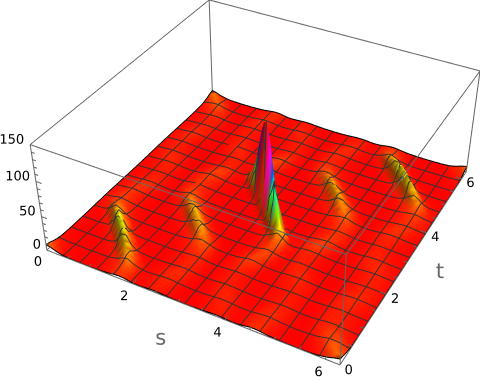
\includegraphics[width=0.7\textwidth]{sections/tangentPointEnergyImgs/kHeatMap1}
        \caption{$k_{2\alpha}^{\alpha}$ heat map}
        \label{fig: Buck-Orloff Heat Map}
    \end{subfigure}
    \caption{Behaviours of $\beta = 2\alpha$ kernel}
\end{figure}



\end{document}
